\documentclass[11pt]{article}
\usepackage{graphicx}
\usepackage{float}
\usepackage{amsmath}
\usepackage{amsfonts}
\usepackage[brazilian]{babel}
\usepackage[utf8]{inputenc}
\usepackage[T1]{fontenc}

%macros
\newcommand{\fromeng}[1]{\footnote{do inglês: \textit{#1}}}
\newcommand{\tit}[1]{\textit{#1}}
\newcommand{\tbf}[1]{\textbf{#1}}
\newcommand{\ttt}[1]{\texttt{#1}}

\begin{document}

\title{MC833 - Tarefa 5}
\author{Erik de Godoy Perillo - RA: 135582}
\maketitle

\begin{enumerate}

\item 
	\begin{enumerate}
		\item \ttt{select(int nfds, fd\_set* readfds, fd\_set* writefds, 
				fd\_set* exceptfds, struct timeval* timeout)}

			A função \ttt{select} monitora grupos de \tit{file descriptors} 
			e indica quais deles estão prontos para uma certa operação
			de I/O. As operações podem ser de leitura (com os \tit{file 
			descriptors} indicados em \ttt{readfds}) ou de escrita 
			(indicados por \ttt{writefds}). Pode-se também indicar um grupo de 
			exceções (indicado por \ttt{exceptfds}). Passa-se o limite superior
			máximo (não-inclusivo) do \tit{range} dos \tit{file descriptors}
			o qual se quer inspecionar pelo argumento \ttt{nfds}. A operação
			pode ter um timeout para um dos \tit{file descriptors} estar 
			disponível especificado em \ttt{timeout}. Se esse argumento
			é NULL, então a função bloqueia até um \tit{file descriptor} 
			estar pronto.
			O gerenciamento dos grupos é feito através de macros:
			
		\item \ttt{FD\_ZERO(set)} - Limpa um grupo.
		\item \ttt{FD\_SET(fd, set)} - 
			Adiciona um file descriptor a um grupo.
		\item \ttt{FD\_CLR(fd, set)} - Remove um file descriptor de um grupo.
		\item \ttt{FD\_ISSET(fd, set)} - Verifica se um file descriptor está em 
			um certo grupo. Essa macro é usada após a chamada de \ttt{select}
			para se averiguar se um certo \tit{file descriptor} está disponível
			para uma certa operação.
	\end{enumerate}

	\item Um console fala mais que mil palavras.
		Na imagem abaixo, o servidor foi invocado à esquerda.
		À direita, invoca-se duas instâncias do echo\_client do trabalho
		3 (compilados para conectar na porta 56789), o telnet e o nc, todos
		conectando ao endereço do servidor. Pode-se ver que todos obtêm
		a resposta esperada (echo) do servidor.

		\begin{figure}[H]
			\centering
			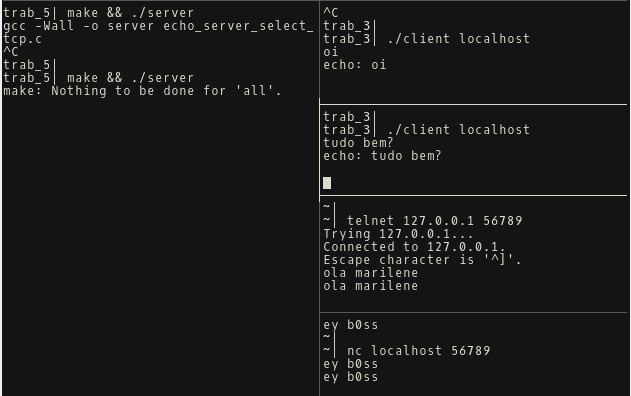
\includegraphics[width=0.9\textwidth]{img/console.png}
		\end{figure}

	\item O truque é obtido por meio de um loop sobre todos os sockets das
		conexões e o uso da função \ttt{select}. No começo de cada loop,
		checa-se se há mais conexões esperando para serem feitas e, se houver,
		uma nova conexão é feita e adicionada à lista de conexões (o vetor
		\ttt{client}). Após isso, itera-se sobre todos os sockets de conexões
		que podem estar ativas. Com o resultado da chamada a \ttt{select} no
		começo do loop e a macro \ttt{FD\_ISSET}, checa-se se o socket analisado
		está disponível para leitura. Se sim, recebe-se uma mensagem e manda-se
		ela de volta. Resumindo: o processo é serial mas, por iterar-se o tempo
		todo sobre os clientes, é dada a impressão de paralelismo.

	\item Foi adicionada checagem de erro para as chamadas de \ttt{select},
		\ttt{accept}, \ttt{read} e \ttt{send}, sempre fechando-se os sockets
		necessários.

	\item A principal diferença é que, para a atividade anterior, era criado
		um processo para cada nova conexão. Na atividade atual, é usado apenas
		um processo para todas as conexões juntamente a um loop infinito que 
		itera sobre todas elas. Com relação a recursos, a abordagem atual
		é mais eficiente pois criar um processo é uma tarefa relativamente
		pesada para o sistema operacional, além de que seria preciso usar um
		\tit{buffer} para cada conexão. Para o que o servidor se propõe a fazer,
		é mais adequado o uso de um processo só, assumindo que não é esperado 
		uma uma interação tão rápida e intensa entre o cliente e o servidor para
		um serviço de echo, além de que é uma tarefa simples que pode ser
		gerenciada facilmente por um único processo. 
		Se muitos usuários conectassem ao servidor que usa \ttt{fork}, haveria
		um problema de escalabilidade muito mais rapidamente que com o servidor
		atual, pois a criação/manipulação de processos pelo sistema operacional
		seria uma tarefa muito mais custosa do que a atividade do echo em si.

\end{enumerate}

\end{document}
